\documentclass[border=8pt]{standalone}

% Visual reference for OpenTikZ layout patterns (reference/layout/layout.md):
% relative placement, index-driven grid distribution, column-fit scaling.
\usepackage{tikz}
\usetikzlibrary{arrows.meta, positioning, fit}

% --- OpenTikZ palette (light / default, Okabe-Ito) ---
\definecolor{otblue}{HTML}{0072B2}
\definecolor{otorange}{HTML}{E69F00}
\definecolor{otteal}{HTML}{009E73}
\definecolor{otpurple}{HTML}{CC79A7}
\definecolor{otgray}{HTML}{5A5A5A}

\begin{document}
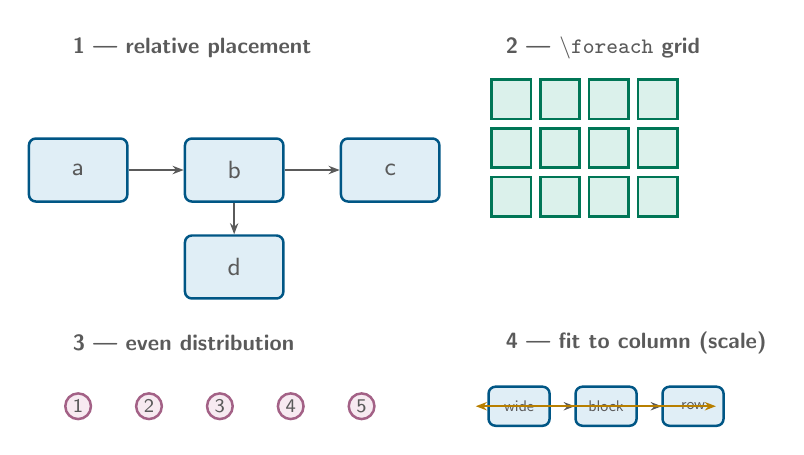
\begin{tikzpicture}[
    line width=0.9pt,
    blk/.style={draw=otblue!75!black, fill=otblue!12, rounded corners=2.5pt,
                minimum width=1.25cm, minimum height=0.8cm, text=otgray,
                font=\sffamily\small},
    cell/.style={draw=otteal!75!black, fill=otteal!14, minimum size=0.5cm},
    caplbl/.style={text=otgray, font=\sffamily\footnotesize\bfseries, anchor=west},
  ]
  % ===== panel 1: relative placement (right=of / below=of) =====
  \node[caplbl] at (-0.2, 1.55) {1 — relative placement};
  \begin{scope}[node distance=4mm and 7mm]
    \node[blk] (a) {a};
    \node[blk, right=of a] (b) {b};
    \node[blk, right=of b] (c) {c};
    \node[blk, below=of b] (d) {d};
    \draw[otgray, -{Stealth[length=4pt]}] (a) -- (b);
    \draw[otgray, -{Stealth[length=4pt]}] (b) -- (c);
    \draw[otgray, -{Stealth[length=4pt]}] (b) -- (d);
  \end{scope}

  % ===== panel 2: index-driven grid =====
  \node[caplbl] at (5.3, 1.55) {2 — \texttt{\textbackslash foreach} grid};
  \begin{scope}[shift={(5.5,0.9)}]
    \def\dx{0.62} \def\dy{0.62}
    \foreach \r in {0,1,2}
      \foreach \cc in {0,1,2,3}
        \node[cell] at (\cc*\dx, -\r*\dy) {};
  \end{scope}

  % ===== panel 3: even distribution across a span =====
  \node[caplbl] at (-0.2, -2.2) {3 — even distribution};
  \begin{scope}[shift={(0,-3.0)}]
    \def\N{5} \def\span{3.6}
    \foreach \i in {1,...,\N}
      \node[circle, draw=otpurple!80!black, fill=otpurple!16, text=otgray,
            font=\sffamily\scriptsize, inner sep=1.2pt]
        at ({(\i-1)/(\N-1)*\span}, 0) {\i};
  \end{scope}

  % ===== panel 4: column-fit scaling (scale + transform shape) =====
  \node[caplbl] at (5.3, -2.2) {4 — fit to column (scale)};
  \begin{scope}[shift={(5.6,-3.0)}, scale=0.62, transform shape,
                node distance=3mm and 5mm]
    \node[blk] (x) {wide};
    \node[blk, right=of x] (y) {block};
    \node[blk, right=of y] (z) {row};
    \draw[otgray, -{Stealth[length=4pt]}] (x) -- (y);
    \draw[otgray, -{Stealth[length=4pt]}] (y) -- (z);
  \end{scope}
  \draw[otorange!80!black, line width=0.8pt, {Stealth[length=4pt]}-{Stealth[length=4pt]}]
    (5.05,-3.0) -- (8.1,-3.0);
\end{tikzpicture}
\end{document}
